%%%%%%%%%%%%%%%%%%%%%%%%%%%%%%%%%%%%%%%%%%%%%%%%%%%%%%%%%%%%%%%%%%%%%%%%
% Preamble
%%%%%%%%%%%%%%%%%%%%%%%%%%%%%%%%%%%%%%%%%%%%%%%%%%%%%%%%%%%%%%%%%%%%%%%%
\documentclass[11pt]{article}
%
% Packages and other includes
% Pagination
\usepackage[letterpaper, margin=1in]{geometry}
\usepackage{emptypage}
\usepackage{xcolor}
%
% Fonts
\usepackage[T1]{fontenc} % best for Western European languages
\usepackage{lmodern} % Latin Modern instead of CM
\usepackage{textcomp} % required to get special symbols
%
% Math
\usepackage{amsmath, amssymb}
\usepackage{braket}
%
% Graphics, floats, tables
\usepackage{graphicx, color, float, array}
%
% Hyperlinks
\usepackage{hyperref}
%
%
% Definitions and settings
% Paragraph indent and spacing
\setlength{\parskip}{0.4\baselineskip}
\setlength{\parindent}{0in}
%
%
% Title, authors, date
\title{\textbf{Midterm answers}}
\date{February 3, 2022}
%
%
%%%%%%%%%%%%%%%%%%%%%%%%%%%%%%%%%%%%%%%%%%%%%%%%%%%%%%%%%%%%%%%%%%%%%%%%
% Main document
%%%%%%%%%%%%%%%%%%%%%%%%%%%%%%%%%%%%%%%%%%%%%%%%%%%%%%%%%%%%%%%%%%%%%%%%
%

\begin{document}

\maketitle

1. \textbf{Barometric Formula} The barometric formula is given by
\begin{equation*}
  P_h = P_0 e^{-\frac{Mgh}{RT}}
\end{equation*}
where $P_h$ is the pressure at height $h$, $P_0$ is the pressure at ground level,
$M$ is the molar mass of air (28.97 g/mol), $R$ is the gas constant, and $T$ is the
temperature. This formula has been used to approximate the elevation of mountains.
Report to 3 significant figures.

(a) A hiker brings a mercury barometer to measure the height of Mount Everest. At the
summit, the hiker reports the barometric pressure to be 253.0 Torr at $-9^\circ\text{C}$.
Use the barometric formula to approximate the height of Mount Everest.

(b) Mount Everest has an official height of 8,485 meters. Is the calculated height in
(a) overestimated or underestimated? Explain potential errors.

(c) Given the barometric pressure in (a), compute the partial pressure of O$_2$(g) at the summit
(P$_{O2}$) assuming that the atmosphere is made of $21\%$ O$_2$. With the oxyhemoglobin dissociation
curve, estimate the percent hemoglobin saturated with O$_2$ assuming that the P$_{\text{O}2}$ in the blood
is equivalent to the P$_{\text{O}2}$ at the summit.

\begin{quote}
  {\color{blue}
    a) $8.50*10^3$ meters

    b) Overestimation. A potential error is that deriving the barometric formula assumes
    a constant temperature. This is not true in reality since temperature decreases
    going higher in altitude.

    c) P(O$_2$)=53.1 torr, around 75.0$\%$ Hb saturation
  }
\end{quote}

2. \textbf{Isothermal Compression} Suppose 1.87 moles of Cl$_2$(g) at $35^\circ\text{C}$ are
compressed isothermally from a volume of 15.0L to 4.79L. Report to 3 significant figures.

(a) Sketch the process on the $PV$ diagram. Define all variables and show what corresponds
to the work ($w$) done on the gas

(b) Compute the work ($w$) and the heat ($q$) in kJ/mol.

(c) What is the final pressure of the gas?

\begin{quote}
  {\color{blue}
    a) 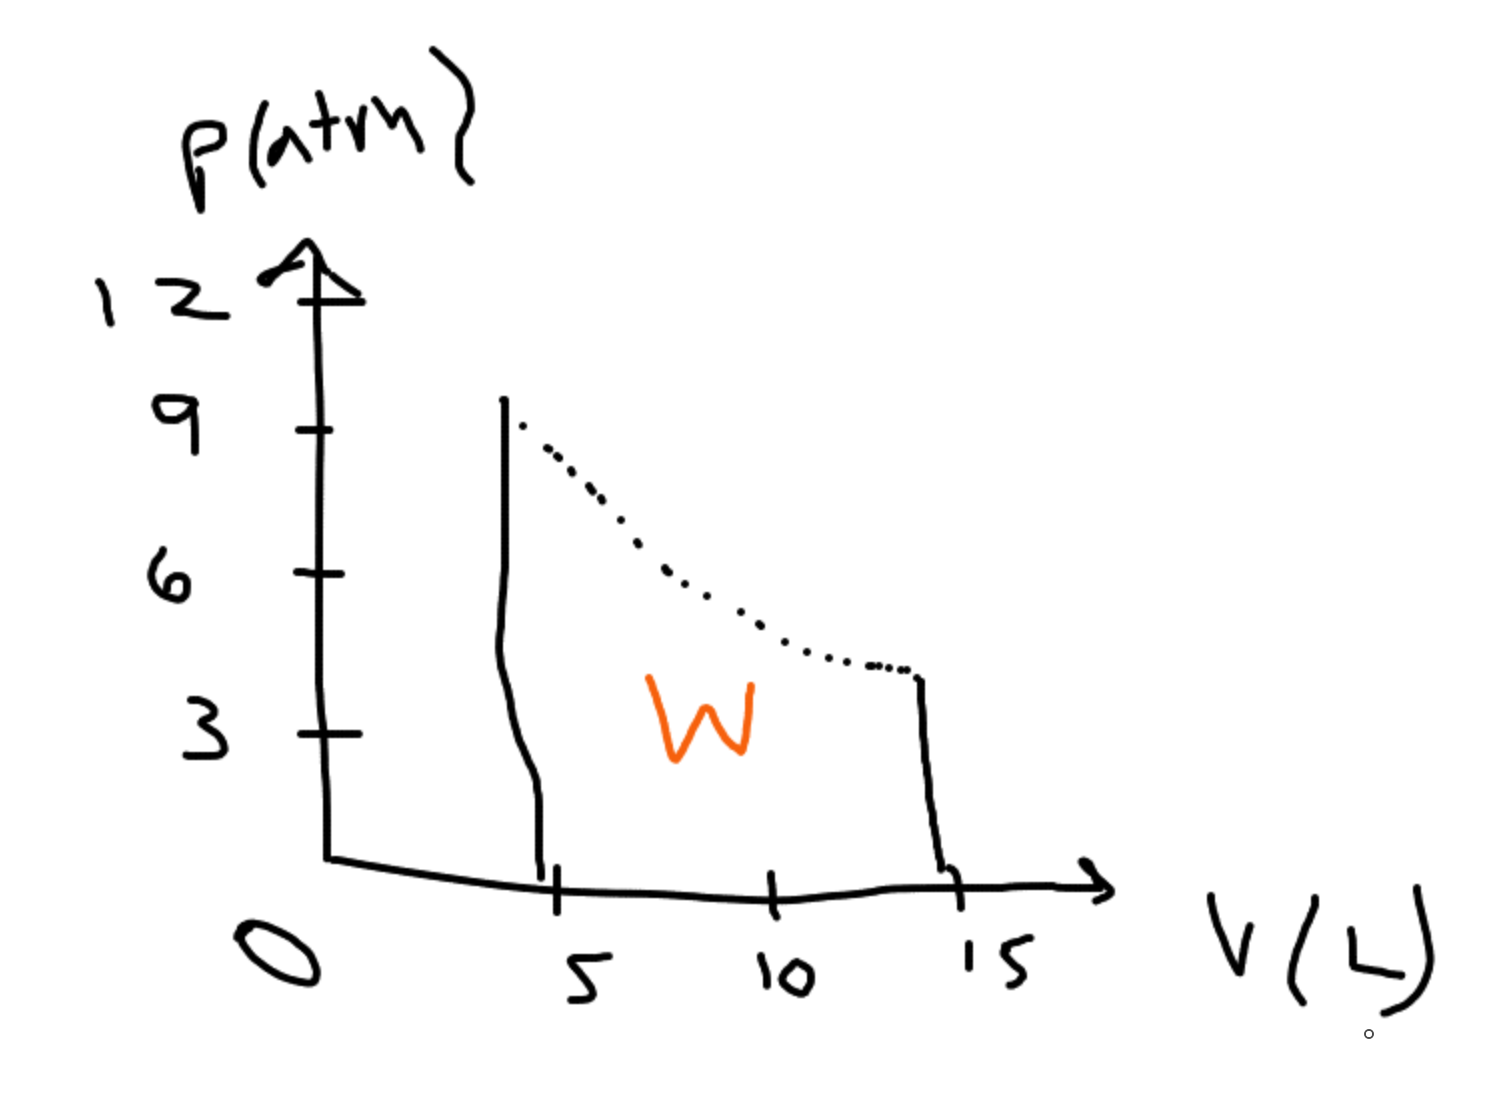
\includegraphics[scale=0.125]{sketch.png}
    
    b) $W = -nRT\ln \frac{V_f}{V_i} =  5470\text{J/mol}$ and $Q=-5470\text{J/mol}$
    
    c) $P= nRT/V_f = 9.87\text{atm}$
  }
\end{quote}

3. \textbf{Decomposition of N$_2$O$_4$(g)} Supposed a sample of N$_2$O$_4$(g) has
a pressure of 6.6 kPa. After some time, a portion of it decomposes to form NO$_2$(g).
The total pressure of the mixture of gases is then 9.8 kPa. Assume the volume and the
temperature do not change. What percentage of N$_2$O$_4$(g) has decomposed? Report to
3 significant figures.

\begin{quote}
  {\color{blue}
    \begin{align}
      PV & = nRT \\
      \frac{P}{n} & = \frac{RT}{V} \\
      \frac{P_1}{n_1} & = \frac{P_2}{n_2} 
    \end{align}

    $P_1$ and $n_1$ are initial while $P_2$ and $n_2$ are the mixture. Determine what $n_2$
    and solve for change. $48.6\%$ decomposed N$_2$O$_4$
    }
\end{quote}

4. Explain in a few sentences what is meant by the ``world energy crisis'' and why
this colloquial term is imprecise in the context of thermodynamics. How is the
``world energy crisis'' related to global warming?

\begin{quote}
  {\color{blue} Mention the 1st law of thermodynamics and greenhouse gases such as
    CO$_2$ leading to less heat escaping the atmosphere.
  }
\end{quote}

5. Quantitative combustion of 1 g of elemental sulfur, S$_8$(s) ($M = 256.48$ g/mol),
to sulfur dioxide gas increases the temperature of a bomb calorimeter from 296 K to
313.5 K. The heat capacity of the calorimeter is 530 J/K. Report all results to 4
significant figures.

a) Formulate a balanced chemical equation for the reaction including states.

b) Determine the energy of reaction.

c) Your result from b) is a good estimate for the standard energy of reaction. Using this
estimate, determine the standard enthalpy of reaction assuming ideal gas behavior.

d) Estimate the standard enthalpy of formation of gaseous sulfur dioxide from these data.

\begin{quote}
  {\color{blue}
    a) S$_8$(s) + 8 O$_2$(g) $\rightarrow$ 8 SO$_2$(g)

    b) $Q = C\Delta T = -9.275\text{kJ}$

    c) $\Delta H_r = \frac{Q}{n_r} = -2379\text{kJ/mol}$

    d) $\Delta H^\circ_f = -297.4\text{kJ/mol}$
  }
\end{quote}

6. A bath tub contains 75 gal of water at a temperature of 110 F, which is scalding hot.
Estimate the volume of 50 F cold tap water needed to bring the temperature to a more
comfortable 104 F. Assume that the bath tub is thermally insulated. Water has a density
of approximately 997 kg/m$^3$ and a specific heat capacity of 4.18 J/(g K).

\begin{quote}
  {\color{blue} $m_h$ is mass (kg) of hot bath, $m_c$ is the mass (kg) of the cold tap
    water, $C$ is heat capacity of water and $\Delta T$ is the change in temperature

    \begin{align}
      m_h C \Delta T_h & = m_c C \Delta T_c \\
      %  m_h \Delta T_h & = m_c \Delta T_c \\
      %  -283.0543*(40 - 43.3333) & = m_c (40 - 10) \\
      m_c & = 31.450446
    \end{align}

    The volume needed is 8.332 galllons of $50^\circ\text{F}$
  }
\end{quote}

\pagebreak

\end{document}
